\begin{figure}[htp]
  \centering
  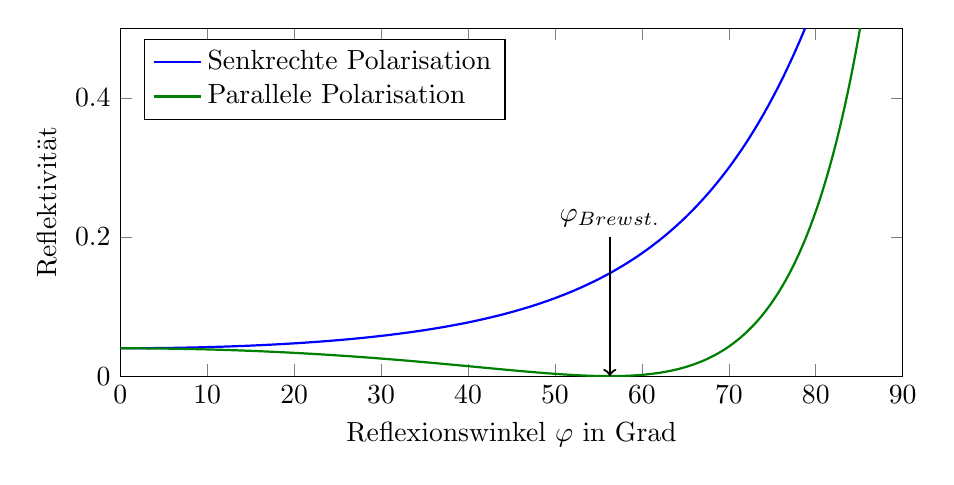
\begin{tikzpicture}
  \begin{axis}[disabledatascaling, width=0.95\textwidth, height=6cm, ylabel=Reflektivität, xlabel=Reflexionswinkel $\varphi$ in Grad, xmin=0, xmax=pi/2, ymin = 0, ymax = .5, samples = 300, domain=0:pi/2, xtick={0,pi/18, pi/9, pi/6, 2*pi/9, 5*pi/18, pi/3, 7*pi/18, 4*pi/9, pi/2}, xticklabels={0,10,20,30,40,50,60,70,80,90}, legend pos=north west, legend cell align={left}]
    \addplot[blue, thick] {((cos(deg(x))-sqrt(2.25-sin(deg(x))^2))/(cos(deg(x))+sqrt(2.25-sin(deg(x))^2)))^2};
    \addplot[green!50!black, thick] {((1.5*cos(deg(x))-sqrt(1-sin(deg(x))^2/2.25))/(1.5*cos(deg(x))+sqrt(1-sin(deg(x))^2/2.25)))^2};
    \legend{Senkrechte Polarisation, Parallele Polarisation};
    \draw[thick, ->] (0.9828,0.2)node[left, anchor=south]{$\varphi_\text{Brewst.}$} -- (0.9828,0);
  \end{axis}
\end{tikzpicture}
  \caption{Reflektivität $R(\varphi)$ als Funktion des Reflexionswinkels $\varphi$ für parallele und senkrechte Polarisation.}
  \label{fig:Reflektivität_Fresnel}
\end{figure}
